\documentclass{article}
\usepackage{tikz}
\usetikzlibrary{shapes.geometric, arrows}
\begin{document}
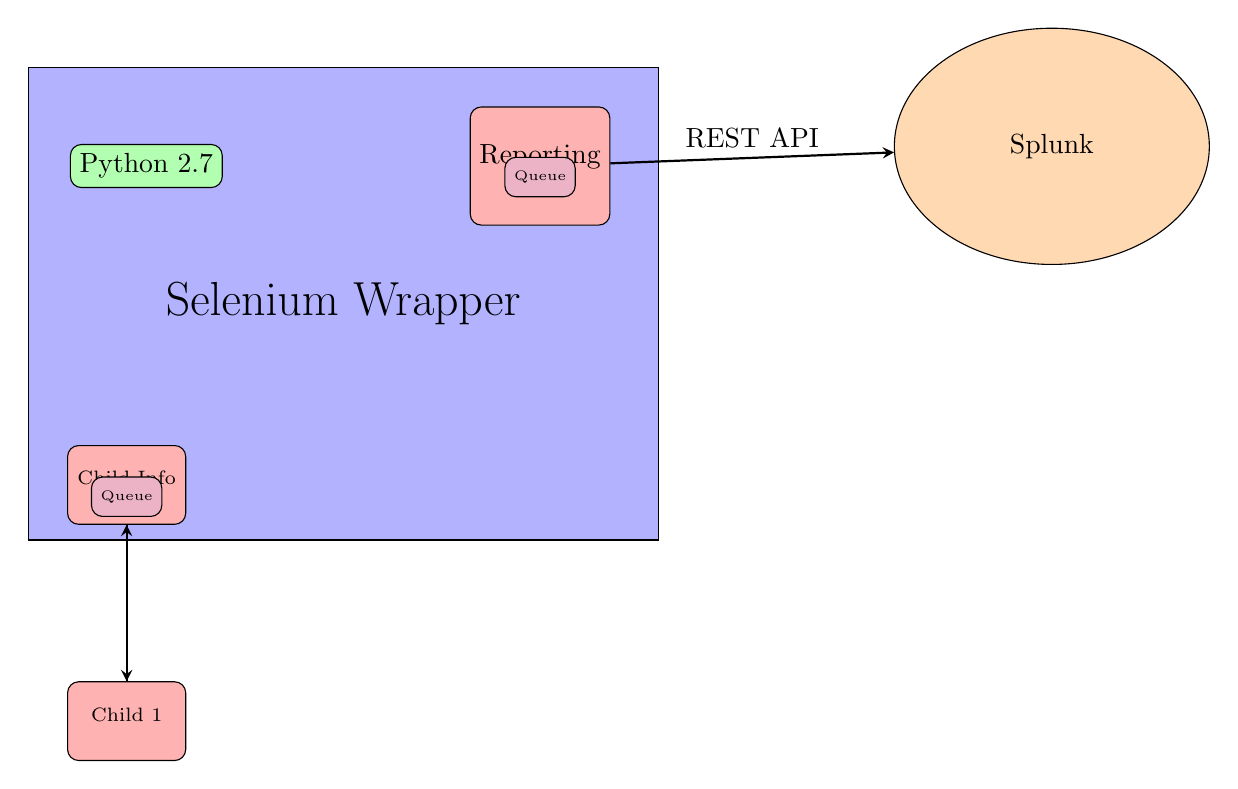
\begin{tikzpicture}

  \tikzstyle{startstop} = [rectangle, rounded corners, minimum width=3cm, minimum height=1cm,text centered, draw=black, fill=red!30]
  \tikzstyle{process} = [rectangle, minimum width=3cm, minimum height=1cm, text centered, draw=black, fill=orange!30]
  \tikzstyle{decision} = [diamond, minimum width=3cm, minimum height=1cm, text centered, draw=black, fill=green!30]

  \tikzstyle{external} = [rectangle, rounded corners, text centered, draw=black, fill=orange!30]
  \tikzstyle{internal} = [rectangle, rounded corners, text centered, draw=black, fill=red!30]
  \tikzstyle{child}    = [internal, minimum height=1cm, minimum width=1.5cm]
  \tikzstyle{q} = [internal, fill=purple!30]

  \tikzstyle{arrow} = [thick,->,>=stealth]

  \node (wrapper) [rectangle, minimum width=8cm, minimum height=6cm, text centered, draw=black, fill=blue!30] {\LARGE Selenium Wrapper};
  \node (python)  [external, fill=green!30, yshift=1.75cm, xshift=-2.5cm] {Python 2.7}; 
  \node (report)  [internal, minimum height=1.5cm, yshift=1.75cm, xshift=2.5cm, text height=-0.75cm] {Reporting}; 
  \node (reportqueue) [q, minimum height=0.5cm, below of=report, yshift=0.86cm] {\tiny Queue};
  
  \node (splunk) [external, right of=wrapper, ellipse, xshift=8cm, yshift=2cm, minimum width=4cm, minimum height=3cm] {Splunk};
  \draw [arrow] (report) -- node[anchor=south] {REST API} (splunk);

  \node (child1data)  [child, below of=wrapper, xshift=-2.75cm, yshift=-1.3cm, text height=-0.5cm ] {\scriptsize Child Info};
  \node (child1queue) [q, minimum height=0.5cm, below of=child1data, yshift=0.85cm] {\tiny Queue};

  \node (child1)      [child, below of=child1data, yshift=-2cm, text height=-0.5cm] {\scriptsize Child 1};
  \draw [arrow] (child1data) -- (child1);
  \draw [arrow] (child1) -- (child1data);
















\end{tikzpicture}
\end{document}
